%!TEX root=../../main.tex

\section{Exercises}

% Chapter 6 exercises
% format adapted from inference_for_means
% problems drawn from OI 4 source files
%__________________
\subsection{Examining scatterplots}

% 1 ODD (OI4, 8.3)

\eoce{\qt{Identify relationships, Part I\label{identify_relationships_1}} 
For each of the six plots, 
identify the strength of the relationship (e.g. weak, moderate, or 
strong) in the data and whether fitting a linear model would be 
reasonable.
\begin{center}
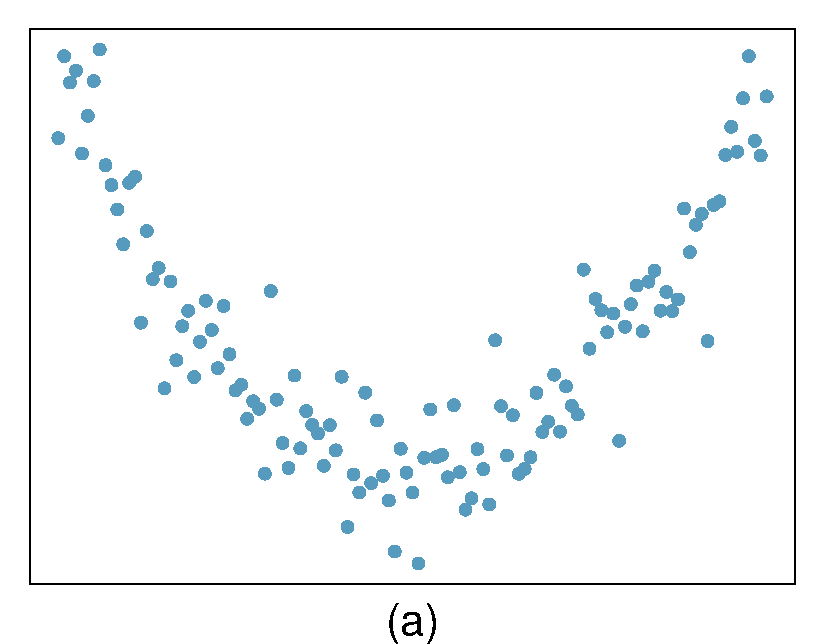
\includegraphics[width=0.32\textwidth]{ch_simple_linear_regression_oi_biostat/figures/eoce/identify_relationships_1/identify_relationships_u.pdf}
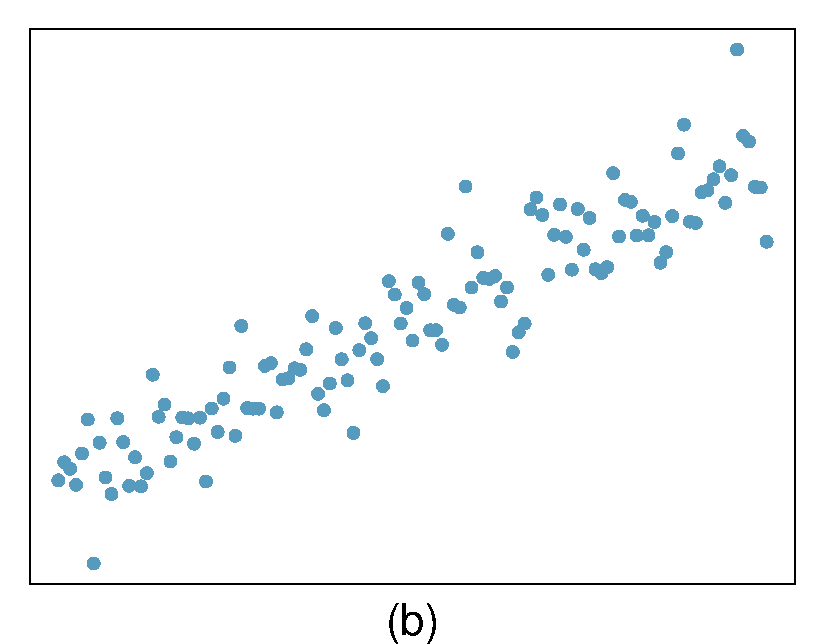
\includegraphics[width=0.32\textwidth]{ch_simple_linear_regression_oi_biostat/figures/eoce/identify_relationships_1/identify_relationships_lin_pos_strong.pdf}
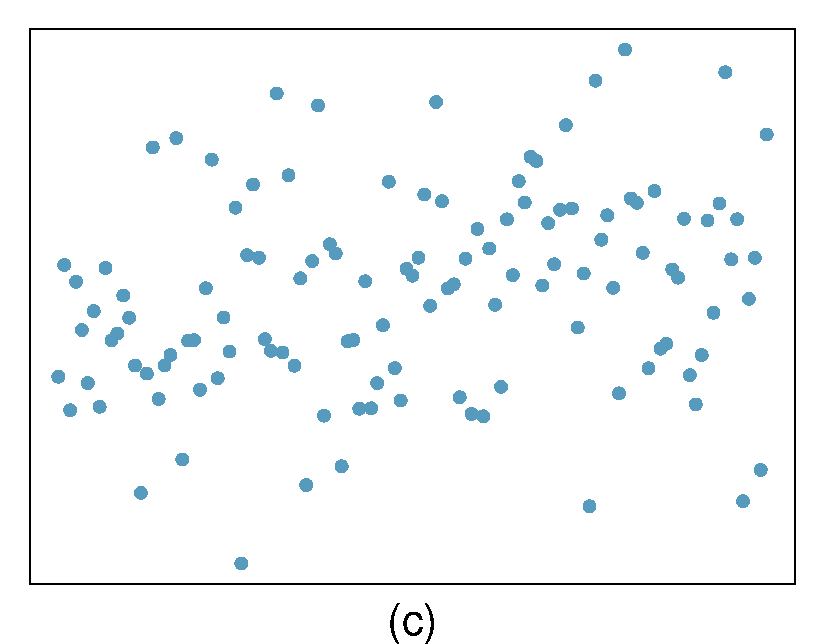
\includegraphics[width=0.32\textwidth]{ch_simple_linear_regression_oi_biostat/figures/eoce/identify_relationships_1/identify_relationships_lin_pos_weak.pdf}
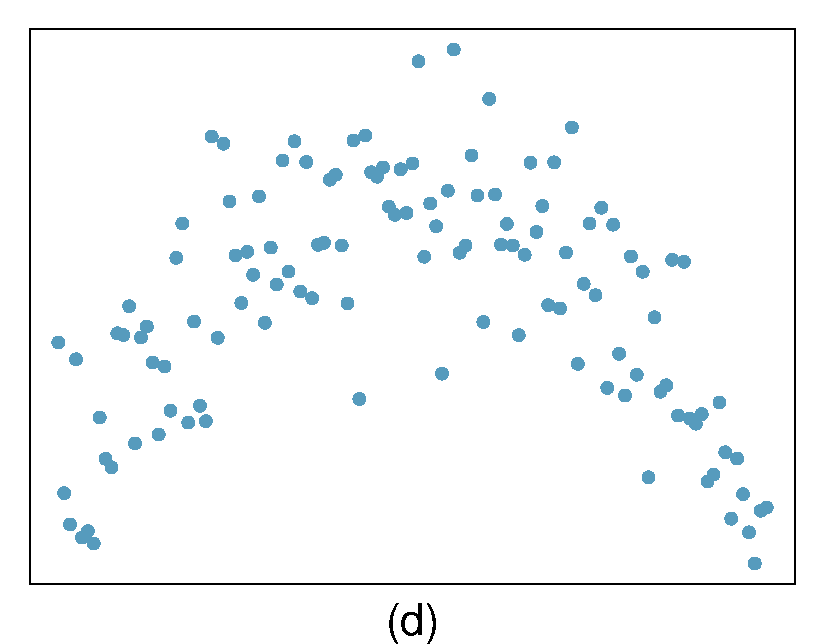
\includegraphics[width=0.32\textwidth]{ch_simple_linear_regression_oi_biostat/figures/eoce/identify_relationships_1/identify_relationships_n.pdf}
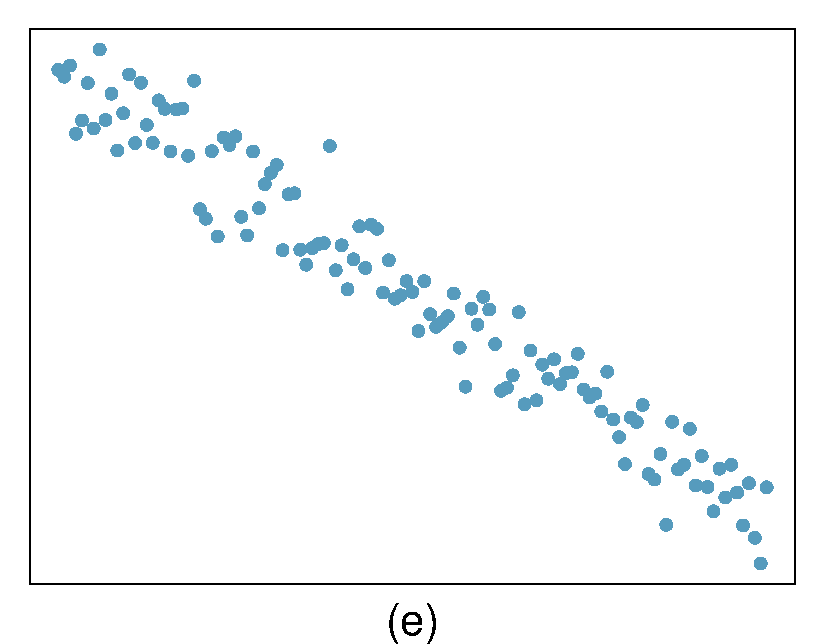
\includegraphics[width=0.32\textwidth]{ch_simple_linear_regression_oi_biostat/figures/eoce/identify_relationships_1/identify_relationships_lin_neg_strong.pdf}
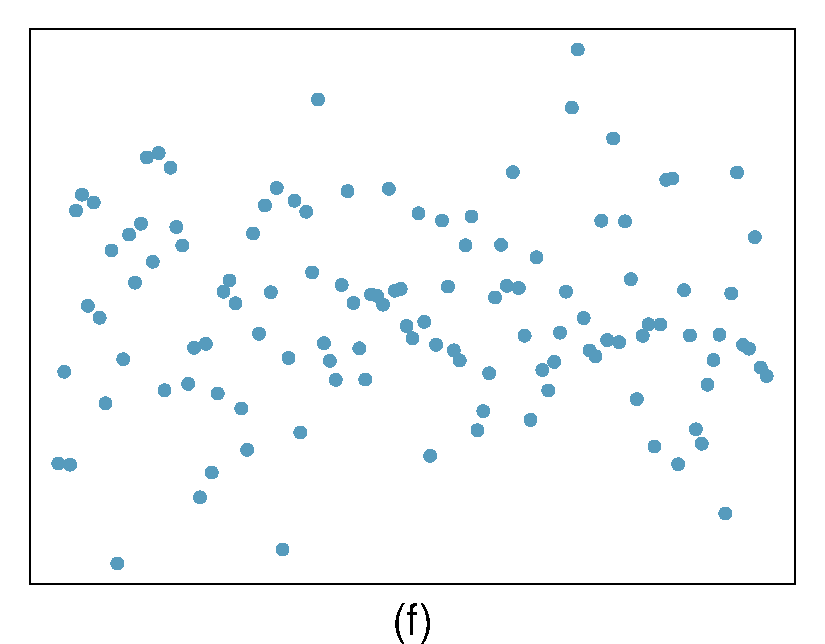
\includegraphics[width=0.32\textwidth]{ch_simple_linear_regression_oi_biostat/figures/eoce/identify_relationships_1/identify_relationships_none.pdf}
\end{center}
}{}

% 2 EVEN (OI4, 8.4)

\eoce{\qt{Identify relationships, Part II\label{identify_relationships_2}} 
For each of the six plots, 
identify the strength of the relationship (e.g. weak, moderate, or 
strong) in the data and whether fitting a linear model would be 
reasonable.
\begin{center}
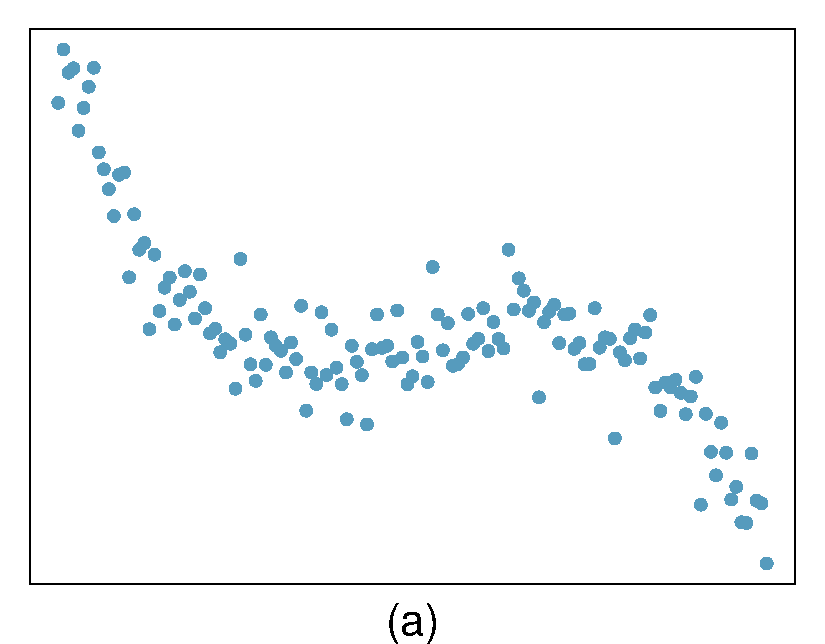
\includegraphics[width=0.32\textwidth]{ch_simple_linear_regression_oi_biostat/figures/eoce/identify_relationships_2/identify_relationships_s.pdf}
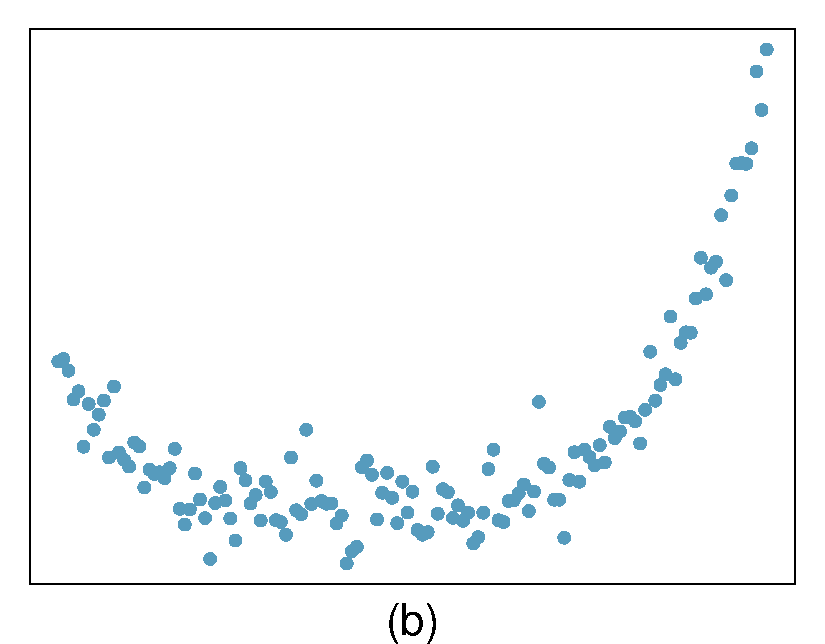
\includegraphics[width=0.32\textwidth]{ch_simple_linear_regression_oi_biostat/figures/eoce/identify_relationships_2/identify_relationships_hockey_stick.pdf}
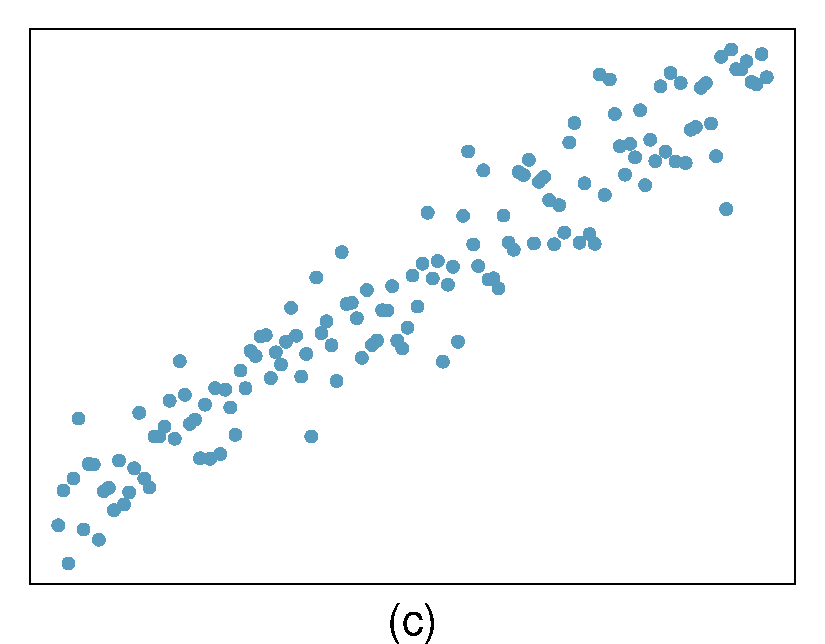
\includegraphics[width=0.32\textwidth]{ch_simple_linear_regression_oi_biostat/figures/eoce/identify_relationships_2/identify_relationships_pos_lin_strong.pdf}
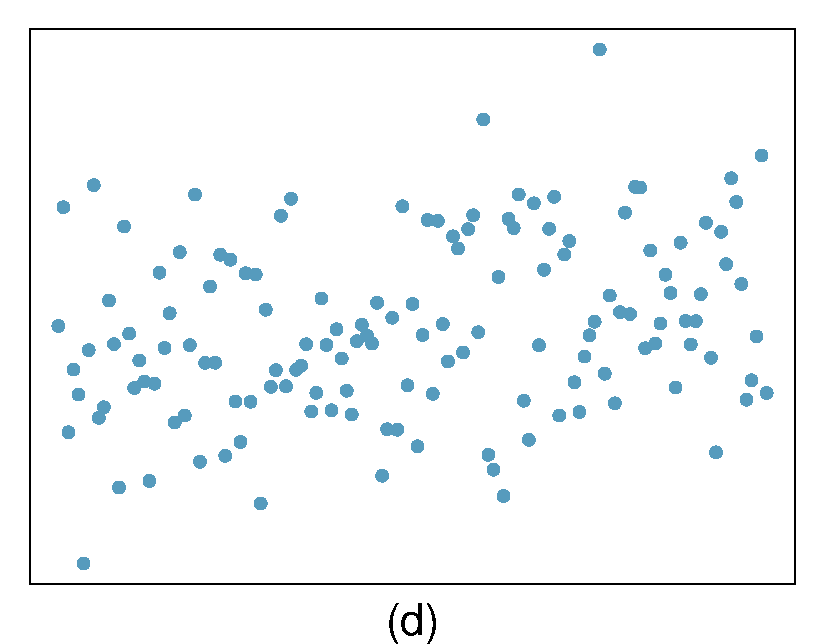
\includegraphics[width=0.32\textwidth]{ch_simple_linear_regression_oi_biostat/figures/eoce/identify_relationships_2/identify_relationships_pos_weak.pdf}
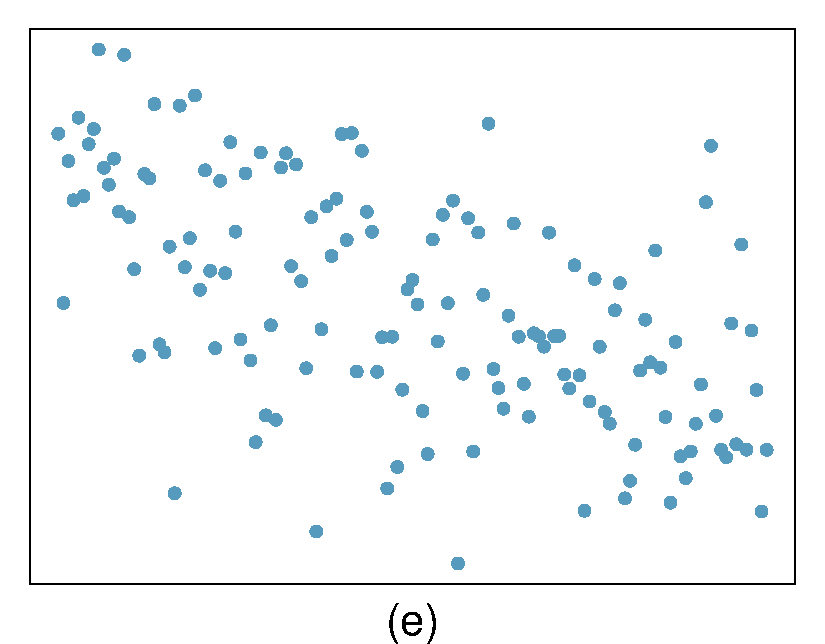
\includegraphics[width=0.32\textwidth]{ch_simple_linear_regression_oi_biostat/figures/eoce/identify_relationships_2/identify_relationships_pos_weaker.pdf}
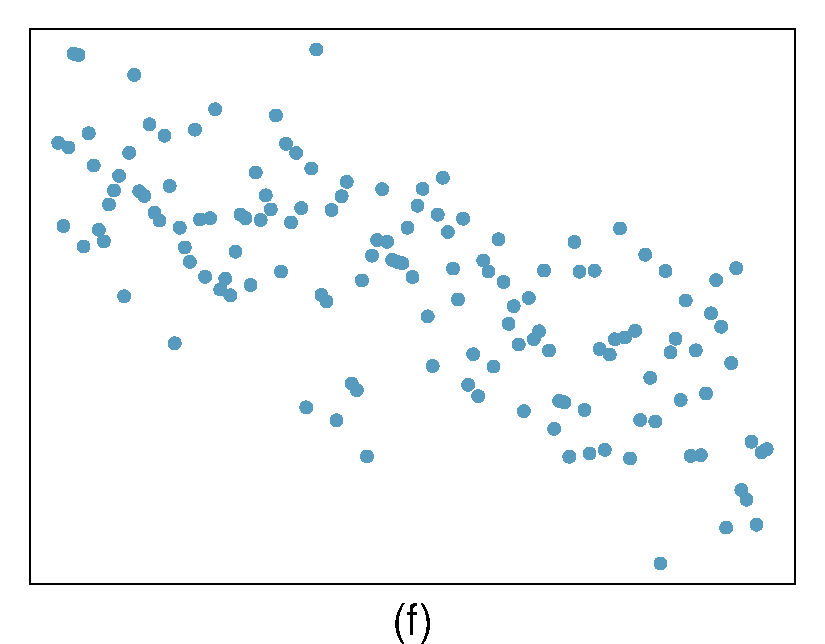
\includegraphics[width=0.32\textwidth]{ch_simple_linear_regression_oi_biostat/figures/eoce/identify_relationships_2/identify_relationships_neg_lin_weak.pdf}
\end{center}
}{}


\textD{\newpage}


\subsection{Estimating a regression line using least squares}

% 3 ODD (OI4, 8.13)

\eoce{\qt{Body measurements, Part I\label{body_measurements_shoulder_height_corr_units}} 
Researchers studying anthropometry collected body girth measurements and 
skeletal diameter measurements, as well as age, weight, height and gender 
for 507 physically active individuals.\footfullcite{Heinz:2003} The 
scatterplot below shows the relationship between height and shoulder 
girth (over deltoid muscles), both measured in centimeters.\vspace{3mm}

\noindent%
\begin{minipage}[c]{0.4\textwidth}
{\raggedright\begin{parts}
\item Describe the relationship between shoulder girth and height.
\item How would the relationship change if shoulder girth was measured 
in inches while the units of height remained in centimeters?
\end{parts}\vspace{20mm}}
\end{minipage}
\begin{minipage}[c]{0.03\textwidth}                  
$\:$\\
\end{minipage}
\begin{minipage}[c]{0.555\textwidth}
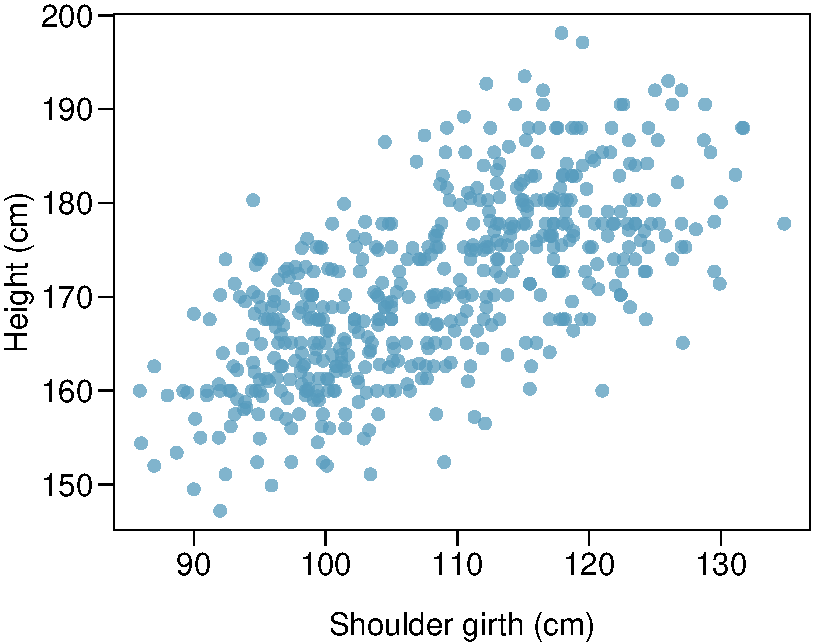
\includegraphics[width=\textwidth]{ch_simple_linear_regression_oi_biostat/figures/eoce/body_measurements_shoulder_height_corr_units/body_measurements_height_shoulder_girth.pdf}
\end{minipage}
}{}


% 4 EVEN (OI4, 8.14)

\eoce{\qt{Body measurements, Part II\label{body_measurements_hip_weight_corr_units}} 
The scatterplot below shows the relationship between weight 
measured in kilograms and hip girth measured in centimeters 
from the data described in 
Exercise~\ref{body_measurements_shoulder_height_corr_units}.%
\vspace{3mm}

\noindent%
\begin{minipage}[c]{0.4\textwidth}
{\raggedright\begin{parts}
\item Describe the relationship between hip girth and weight.
\item How would the relationship change if weight was measured in pounds 
while the units for hip girth remained in centimeters?
\end{parts}\vspace{20mm}}
\end{minipage}
\begin{minipage}[c]{0.03\textwidth}
$\:$\\
\end{minipage}
\begin{minipage}[c]{0.555\textwidth}
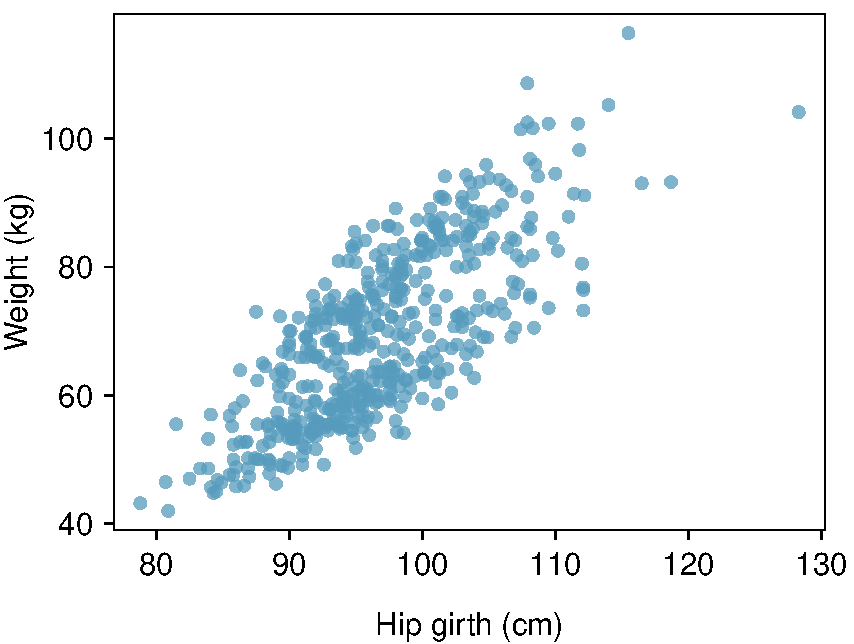
\includegraphics[width=\textwidth]{ch_simple_linear_regression_oi_biostat/figures/eoce/body_measurements_hip_weight_corr_units/body_measurements_weight_hip_girth.pdf}
\end{minipage}
}{}

\textD{\newpage}

% 5 ODD (OI4, 8.19)

\eoce{\qt{Over-under, Part I\label{residual_apple_weight}} Suppose we fit a 
regression line to predict the shelf life of an apple based on its weight. 
For a particular apple, we predict the shelf life to be 4.6 days. The 
apple's residual is -0.6 days. Did we over or under estimate the 
shelf-life of the apple? Explain your reasoning.
}{}

% 6 EVEN (OI4, 8.20)

\eoce{\qt{Over-under, Part II\label{residual_sun_cancer}} Suppose we fit a 
regression line to predict the number of incidents of skin cancer per 
1,000 people from the number of sunny days in a year. For a particular 
year, we predict the incidence of skin cancer to be 1.5 per 1,000 people, 
and the residual for this year is 0.5. Did we over or under estimate 
the incidence of skin cancer? Explain your reasoning.
}{}

% 7 ODD (OI, 8.25) edited

\eoce{\qt{Murders and poverty, Part I\label{murders_poverty_reg}} The following 
	regression output is for predicting annual murders per million from 
	percentage living in poverty in a random sample of 20 metropolitan 
	areas.\\[2mm]
	\begin{minipage}[c]{0.5\textwidth}
		{\footnotesize
			\begin{tabular}{rrrrr}
				\hline
				& Estimate  & Std. Error    & t value   & Pr($>$$|$t$|$) \\ 
				\hline
				(Intercept) & -29.901   & 7.789         & -3.839    & 0.001 \\ 
				poverty\%   & 2.559     & 0.390         & 6.562     & 0.000 \\ 
				\hline
			\end{tabular} \\
			$s = 5.512 \hfill R^2 = 70.52\% \hfill R^2_{adj} = 68.89\%$ 
		}
		\begin{parts}
			\item Write out the linear model.
			\item Interpret the intercept.
			\item Interpret the slope.
			%\item Interpret $R^2$.
			\item Calculate the correlation coefficient.
		\end{parts}
	\end{minipage}
	\begin{minipage}[c]{0.02\textwidth}
		$\:$\\
	\end{minipage}
	\begin{minipage}[c]{0.45\textwidth}
		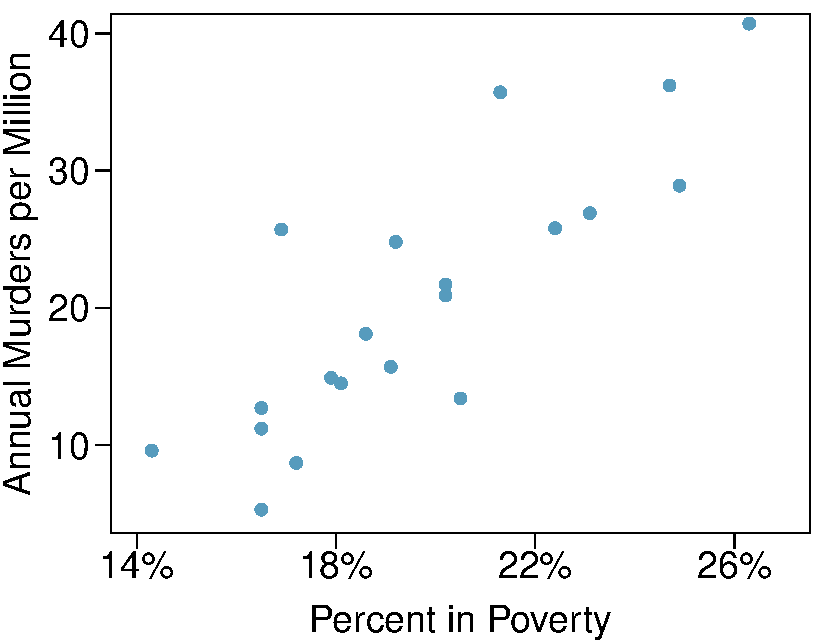
\includegraphics[width=\textwidth]{ch_simple_linear_regression_oi_biostat/figures/eoce/murders_poverty_reg/murders_poverty.pdf}
	\end{minipage}
}{}


% 8 EVEN (OI4, 8.26) edited

\eoce{\qt{Cats, Part I\label{cat_body_heart_reg}} The following regression output is 
	for predicting the heart weight (in g) of cats from their body weight 
	(in kg). The coefficients are estimated using a dataset of 144 
	domestic cats.\\[2mm]
	\begin{minipage}[c]{0.5\textwidth}
		{\footnotesize
			\begin{tabular}{rrrrr}
				\hline
				& Estimate  & Std. Error    & t value   & Pr($>$$|$t$|$) \\ 
				\hline
				(Intercept) & -0.357    & 0.692         & -0.515    & 0.607 \\ 
				body wt     & 4.034     & 0.250         & 16.119    & 0.000 \\ 
				\hline
			\end{tabular} \\
			$s = 1.452 \hfill R^2 = 64.66\% \hfill R^2_{adj} = 64.41\%$ 
		}
		\begin{parts}
			\item Write out the linear model.
			\item Interpret the intercept.
			\item Interpret the slope.
			%\item Interpret $R^2$.
			\item Calculate the correlation coefficient.
		\end{parts}
	\end{minipage}
	\begin{minipage}[c]{0.02\textwidth}
		$\:$\\
	\end{minipage}
	\begin{minipage}[c]{0.45\textwidth}
		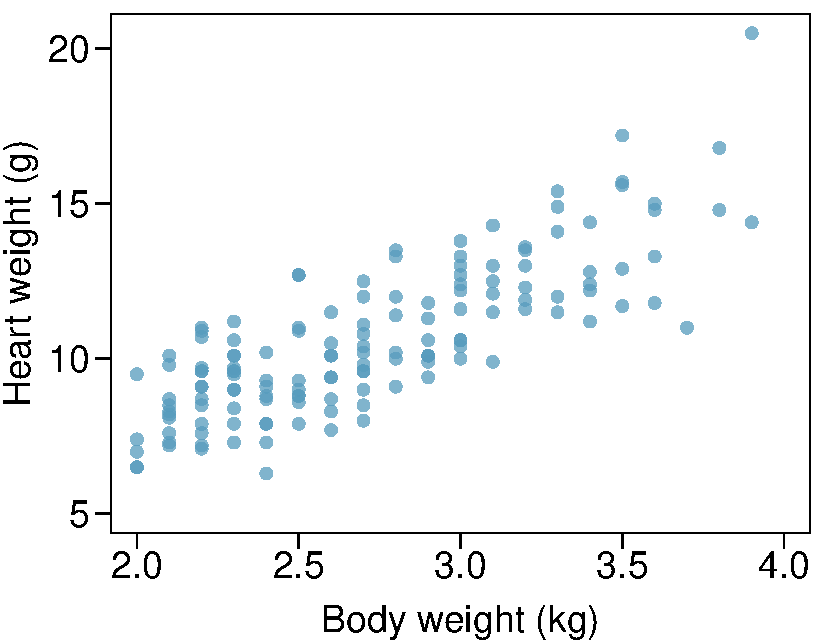
\includegraphics[width=\textwidth]{ch_simple_linear_regression_oi_biostat/figures/eoce/cat_body_heart_reg/cat_body_heart.pdf}
	\end{minipage}
}{}

\textD{\newpage}

% 9 oi_biostat, from lab 6.1

\eoce{\qt{Age and RFFT score, Part I\label{age_rfft_lm}} A linear model fit to RFFT scores and age for 500 randomly sampled individuals from the PREVEND data has equation $\widehat{RFFT} = 137.55 - 1.26(Age)$.
	
\begin{parts}
	\item Interpret the slope and intercept values in the context of the data; i.e., explain the linear model in terms that a non-statistician would understand. Comment on whether the intercept value has any interpretive meaning in this setting.
	
	\item Based on the linear model, how much does RFFT score differ, on average, between an individual who is 60 years old versus an individual who is 50 years old?
	
	\item According to the linear model, what is the average RFFT score for an individual who is 70 years old?
	
	\item Examine Figure~\ref{prevendAgeRFFT}. Is it valid to use the linear model to estimate RFFT score for an individual who is 20 years old? Explain your answer.
	
\end{parts}

}{}

% 10 oi_biostat, from section 6, spring 2020

\eoce{\qt{Guppies, Part I\label{guppies_one}} Guppies are small, brightly colored tropical fish often seen in freshwater fish aquariums. A study was conducted in 147 male guppies to examine the relationship between coloration and heterozygosity; heterozygosity refers to the condition of having different alleles at a given genetic locus. The guppies were randomly sampled from a river in the wild.
	
In an initial stage of the study, researchers examined whether length and height are linearly associated. The mean length is 1261.21 cm, with standard deviation 95.62 cm. The mean height is 201.75 cm, with standard deviation 20.68. The correlation between length and height is 0.85. \\[3mm]	

\noindent%
\begin{minipage}[c]{0.4\textwidth}
	{\raggedright\begin{parts}
			\item From a visual inspection, does it seem like the line is a reasonable fit for the data?
			\item Write the equation of the regression line for predicting length from height.
			\item Estimate the predicted mean length of a guppy with height 180 cm.
		\end{parts}\vspace{20mm}}
\end{minipage}
\begin{minipage}[c]{0.02\textwidth}                  
	$\:$\\
\end{minipage}
\begin{minipage}[c]{0.565\textwidth}
	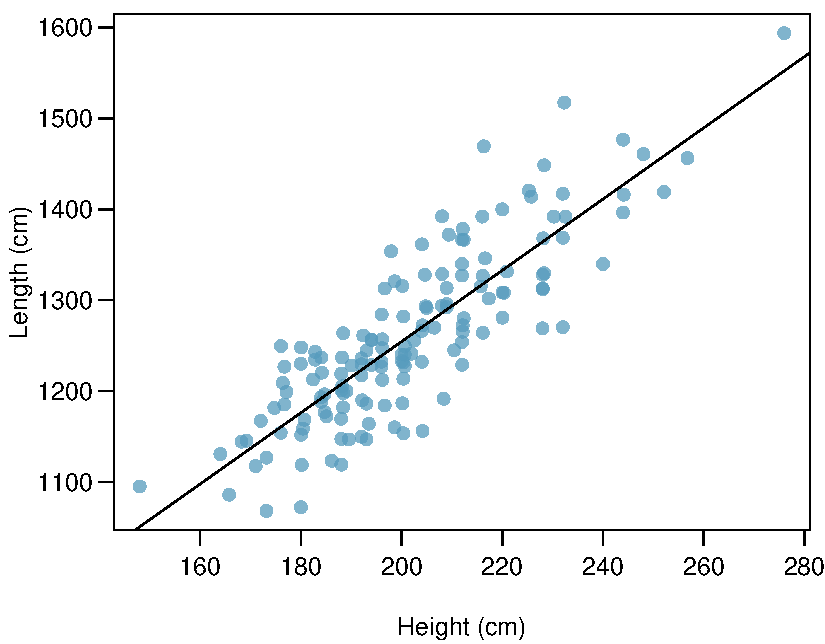
\includegraphics[width=\textwidth]{ch_simple_linear_regression_oi_biostat/figures/eoce/guppies/guppies_length_height.pdf}
\end{minipage}
	
}{}


\textD{\newpage}


\subsection{Interpreting a linear model}

% 11 ODD (OI4, 8.1)

\eoce{\qt{Visualize the residuals\label{visualize_residuals}} 
	The scatterplots shown below each have a 
	superimposed regression line. If we were to construct a residual plot 
	(residuals versus $x$) for each, describe what those plots would look 
	like.
	\begin{center}
		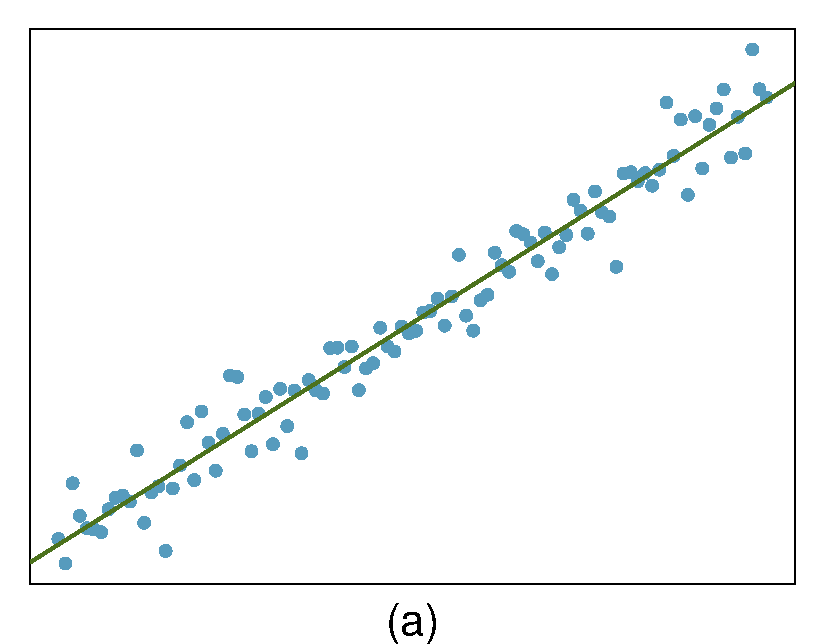
\includegraphics[width=0.44\textwidth]{ch_simple_linear_regression_oi_biostat/figures/eoce/visualize_residuals/visualize_residuals_linear.pdf} 
		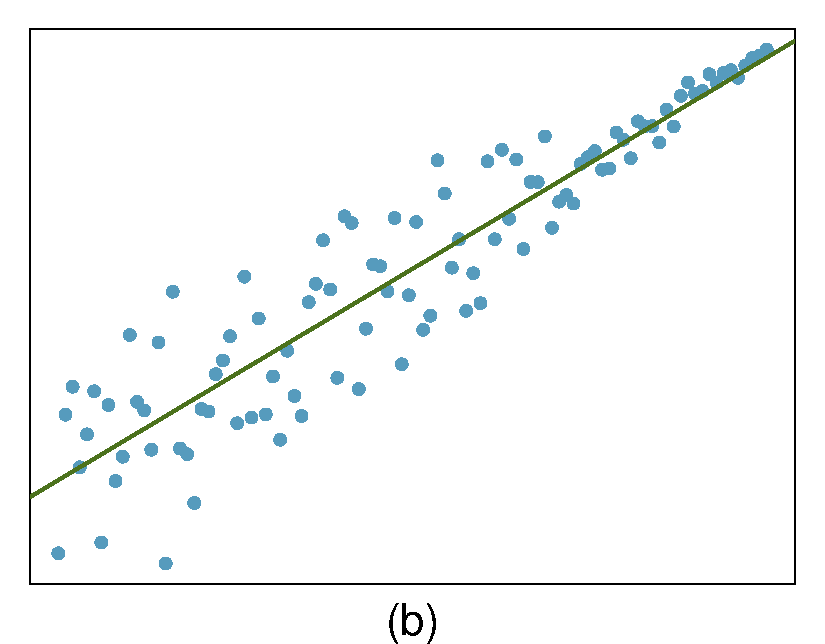
\includegraphics[width=0.44\textwidth]{ch_simple_linear_regression_oi_biostat/figures/eoce/visualize_residuals/visualize_residuals_fan_back.pdf}
	\end{center}
}{}

% 12 (OI4, 8.2)

\eoce{\qt{Trends in the residuals\label{trends_in_residuals}} 
	Shown below are two plots of residuals 
	remaining after fitting a linear model to two different sets of data. 
	Describe important features and determine if a linear model would be 
	appropriate for these data. Explain your reasoning.
	\begin{center}
		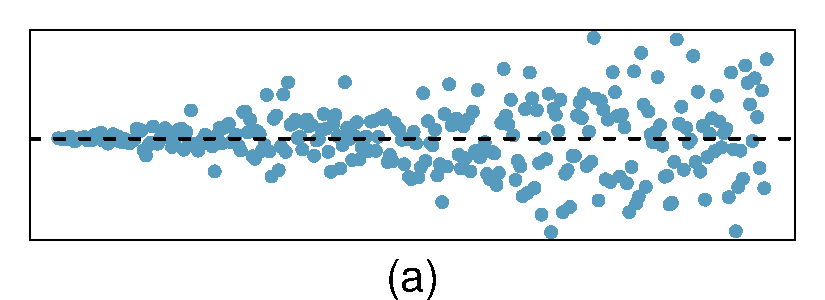
\includegraphics[width=0.44\textwidth]{ch_simple_linear_regression_oi_biostat/figures/eoce/trends_in_residuals/trends_in_residuals_fan.pdf} 
		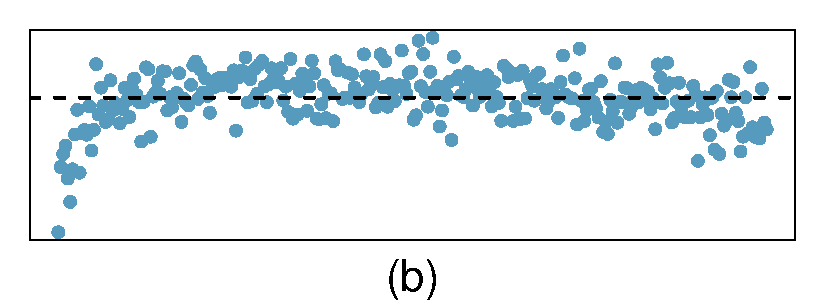
\includegraphics[width=0.44\textwidth]{ch_simple_linear_regression_oi_biostat/figures/eoce/trends_in_residuals/trends_in_residuals_log.pdf}
	\end{center}
}{}

% 13 oi_biostat

\eoce{\qt{Guppies, Part II\label{guppies_influential}} Exercise~\ref{guppies_one} showed a plot of length versus height for 147 male guppies with a least squares regression line. 
	\begin{parts}
	\item Identify two points that have relatively high leverage and discuss whether these points seem to be particularly influential.
	
	\item Based on the plot, comment on whether it is appropriate to use $R^2$ as a metric for describing the strength of the model fit.
	
	\item The $R^2$ for this model is 0.718. Interpret this value in the context of the data.
	
	\end{parts}
}{}

\textD{\newpage}

% 14 EVEN (OI4, 8.22)

\eoce{\qt{Nutrition at Starbucks, Part I\label{starbucks_cals_carbos}} 
	The scatterplot below shows the relationship between the number of 
	calories and amount of carbohydrates (in grams) Starbucks food menu 
	items contain.\footfullcite{data:starbucksCals} Since Starbucks only 
	lists the number of calories on the display items, we are interested 
	in predicting the amount of carbs a menu item has based on its 
	calorie content.
	\begin{center}
		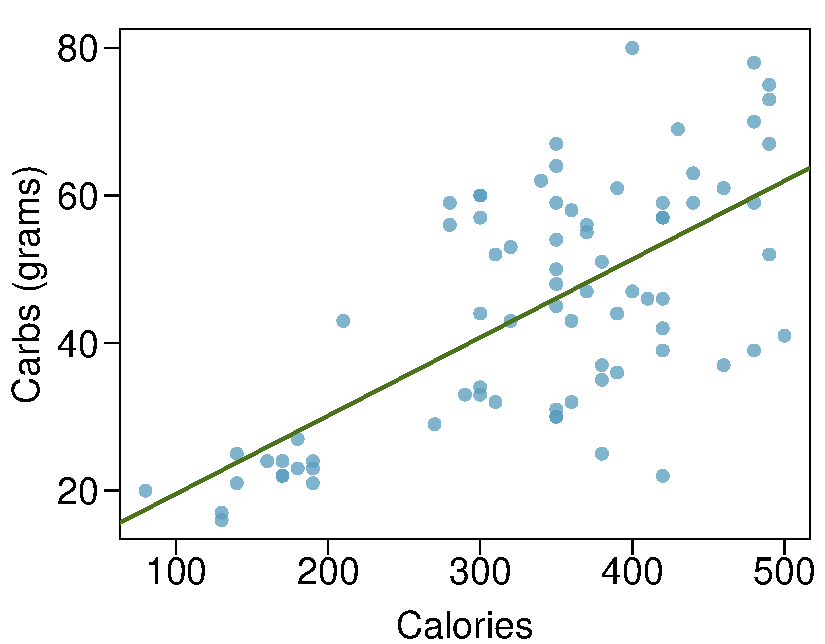
\includegraphics[width=0.32\textwidth]{ch_simple_linear_regression_oi_biostat/figures/eoce/starbucks_cals_carbos/starbucks_cals_carbos.pdf}
		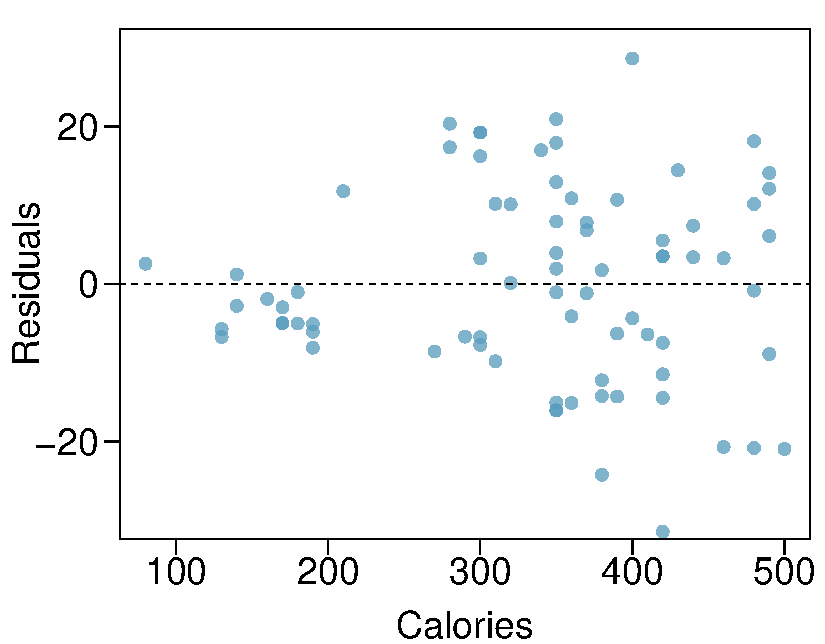
\includegraphics[width=0.32\textwidth]{ch_simple_linear_regression_oi_biostat/figures/eoce/starbucks_cals_carbos/starbucks_cals_carbos_residuals.pdf}
		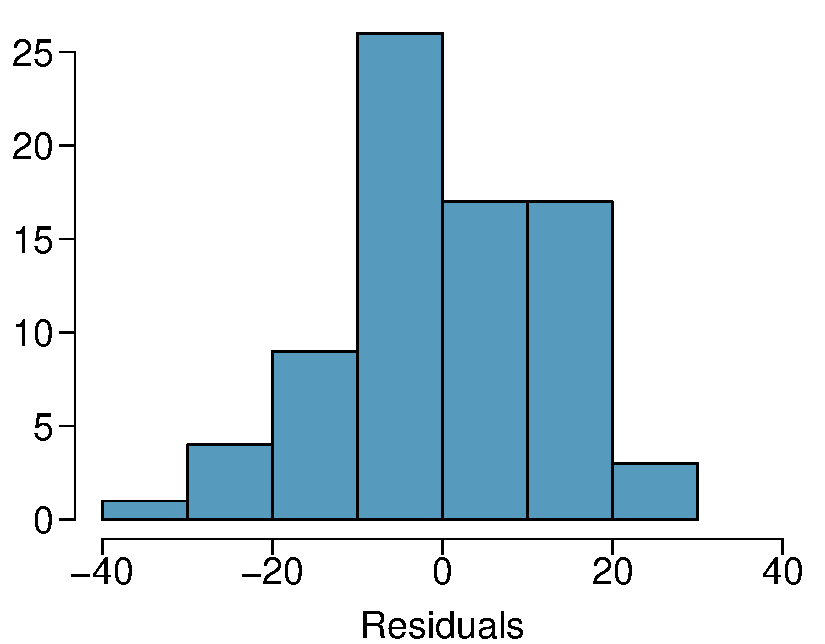
\includegraphics[width=0.32\textwidth]{ch_simple_linear_regression_oi_biostat/figures/eoce/starbucks_cals_carbos/starbucks_cals_carbos_residuals_hist.pdf}
	\end{center}
	\begin{parts}
		\item Describe the relationship between number of calories and amount 
		of carbohydrates (in grams) that Starbucks food menu items contain.
		\item In this scenario, what are the explanatory and response 
		variables?
		\item Why might we want to fit a regression line to these data?
		\item Do these data meet the conditions required for fitting a least 
		squares line?
	\end{parts}
}{}

% 15 ODD (OI4, 8.41)

\eoce{\qt{Nutrition at Starbucks, Part II\label{starbucks_cals_protein}} 
	Exercise~\ref{starbucks_cals_carbos} introduced a data set on nutrition 
	information on Starbucks food menu items. Based on the scatterplot 
	and the residual plot provided, describe the relationship between the 
	protein content and calories of these menu items, and determine if a 
	simple linear model is appropriate to predict amount of protein from 
	the number of calories.
	\begin{center}
		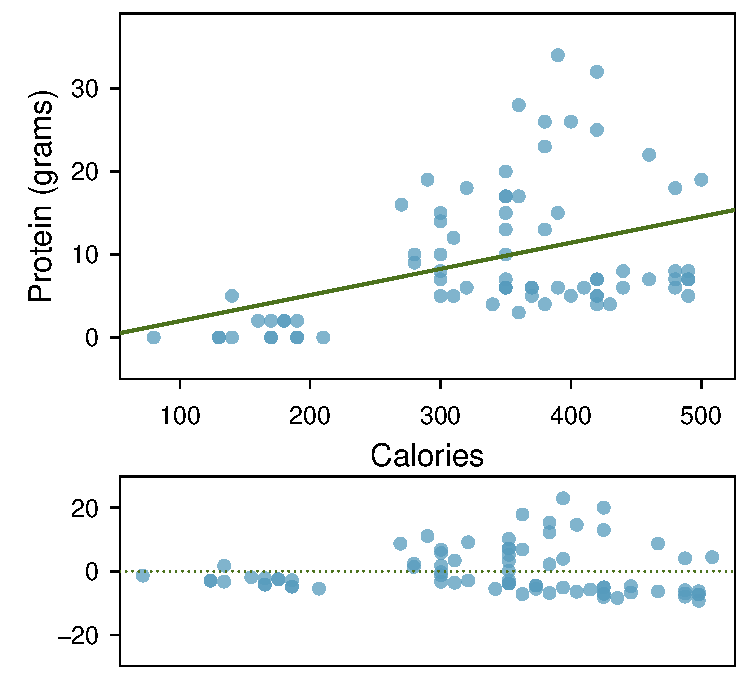
\includegraphics[width=0.6\textwidth]{ch_simple_linear_regression_oi_biostat/figures/eoce/starbucks_cals_protein/starbucks_cals_protein}
	\end{center}
}{}

\textD{\newpage}

% 16 EVEN (OI4, 8.24)

\eoce{\qt{Body measurements, Part III\label{body_measurements_shoulder_height_reg}}
Exercise~\ref{body_measurements_shoulder_height_corr_units} introduces 
data on shoulder girth and height of a group of individuals. The 
mean shoulder girth is 107.20 cm with a standard deviation of 
10.37 cm. The mean height is 171.14 cm with a standard deviation 
of 9.41 cm. The correlation between height and shoulder girth is 0.67.
\begin{parts}
\item Write the equation of the regression line for predicting height.
\item Interpret the slope and the intercept in this context.
\item Calculate $R^2$ of the regression line for predicting height 
from shoulder girth, and interpret it in the context of the 
application.
\item A randomly selected student from your class has a shoulder 
girth of 100 cm. Predict the height of this student using the model.
\item The student from part~(d) is 160 cm tall. Calculate the 
residual, and explain what this residual means.
\item A one year old has a shoulder girth of 56 cm. Would it be 
appropriate to use this linear model to predict the height of this 
child?
\end{parts}
}{}

% 17 ODD (OI4, 8.27)

\eoce{\qt{Outliers, Part I\label{outliers_1}} Identify the outliers in the 
scatterplots shown below, and determine what type of outliers they are. 
Explain your reasoning.
\begin{center}
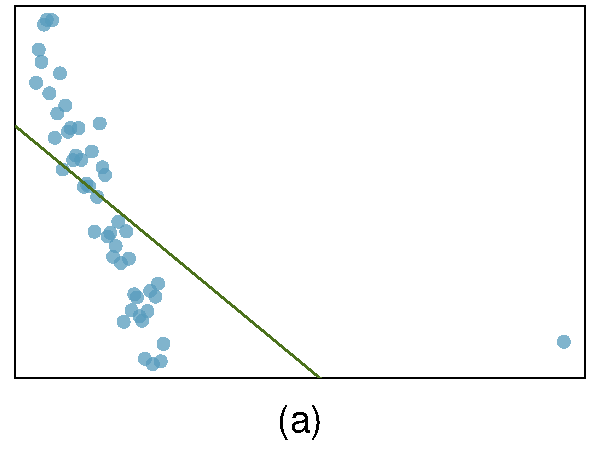
\includegraphics[width=0.32\textwidth]{ch_simple_linear_regression_oi_biostat/figures/eoce/outliers_1/outliers_1_influential.pdf}
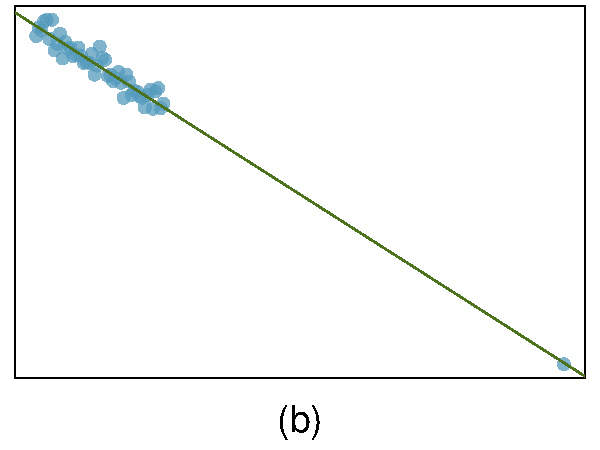
\includegraphics[width=0.32\textwidth]{ch_simple_linear_regression_oi_biostat/figures/eoce/outliers_1/outliers_2_leverage.pdf}
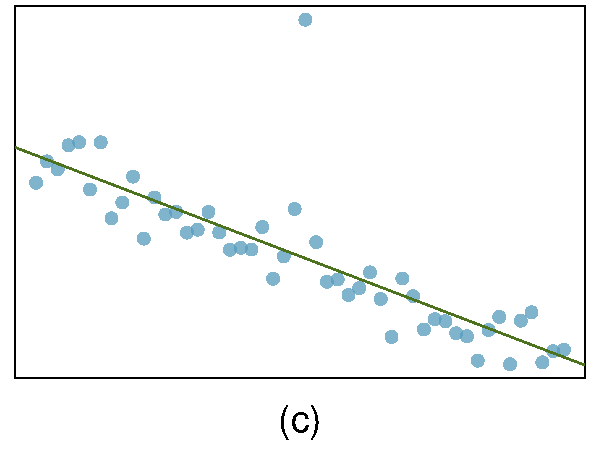
\includegraphics[width=0.32\textwidth]{ch_simple_linear_regression_oi_biostat/figures/eoce/outliers_1/outliers_3_outlier.pdf}
\end{center}
}{}

% 18 EVEN (OI4, 8.28)

\eoce{\qt{Outliers, Part II\label{outliers_2}} Identify the outliers in the scatterplots 
shown below and determine what type of outliers they are. Explain 
your reasoning.
\begin{center}
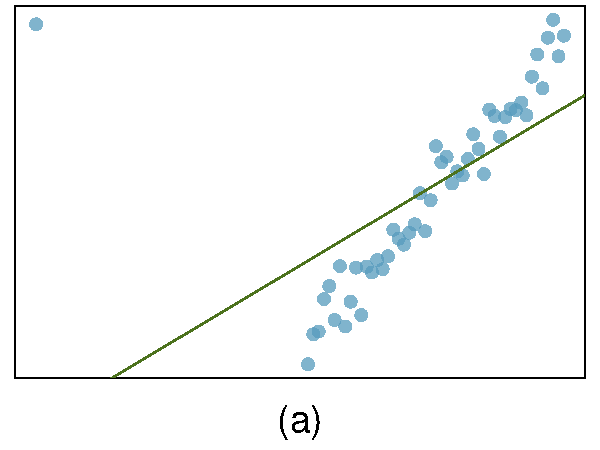
\includegraphics[width=0.32\textwidth]{ch_simple_linear_regression_oi_biostat/figures/eoce/outliers_2/outliers_1_influential.pdf}
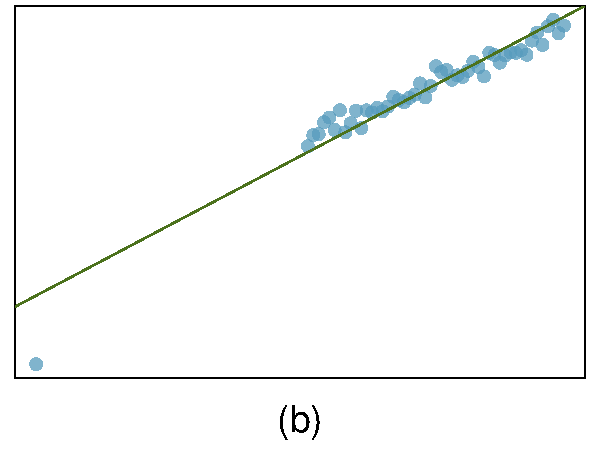
\includegraphics[width=0.32\textwidth]{ch_simple_linear_regression_oi_biostat/figures/eoce/outliers_2/outliers_2_influential.pdf}
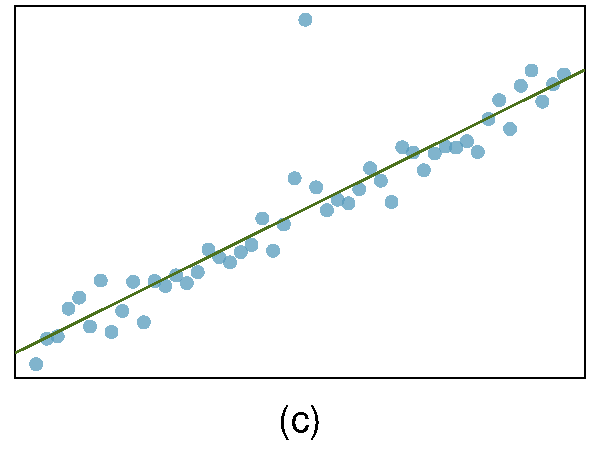
\includegraphics[width=0.32\textwidth]{ch_simple_linear_regression_oi_biostat/figures/eoce/outliers_2/outliers_3_outlier.pdf}
\end{center}
}{}

\textD{\newpage}

% 19 oi_biostat

\eoce{\qt{Guppies, Part III\label{guppies_assumptions}} The residual plots below are for the linear model fit in Exercise~\ref{guppies_one} predicting length from height for 147 male guppies.
\begin{center}
	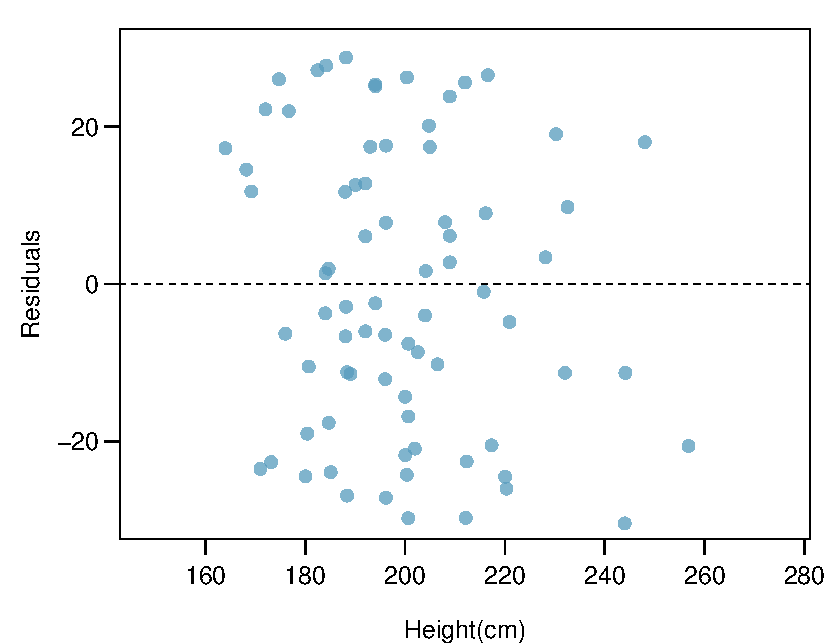
\includegraphics[width=0.485\textwidth]{ch_simple_linear_regression_oi_biostat/figures/eoce/guppies/guppies_resid.pdf}
	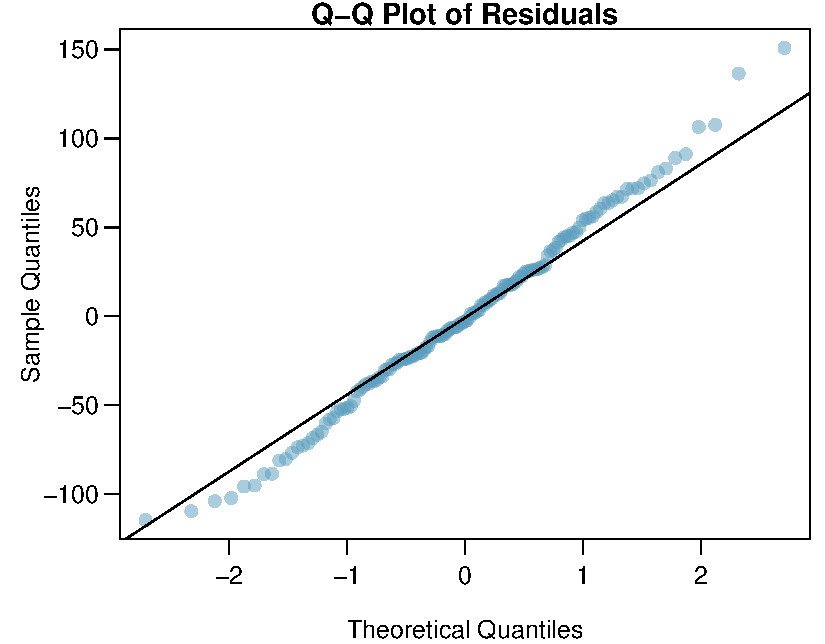
\includegraphics[width=0.485\textwidth]{ch_simple_linear_regression_oi_biostat/figures/eoce/guppies/guppies_qq.pdf}
\end{center}	

\begin{parts}
	\item From a plot of residual values versus predicted values, are the assumptions of linearity and constant variability satisfied? Explain your answer.
	\item Is it reasonable to assume that the observations were independent, based on the description of the study? Explain your answer.
	\item Are the residuals approximately normally distributed? Explain your answer.
\end{parts}
	
}{}

% 20 oi_biostat

\eoce{\qt{Guppies, Part IV\label{guppies_mlh}} Multilocus heterozygosity (MLH) is reflective of genetic quality; according to sexual selection research, it is thought that sexual ornamentation functions as a visual indicator of fitness. By selecting males with features such as bright coloration, females can improve the chances of reproductive success. 
	
	Male guppies are covered in a mixture of colored spots; orange coloration is consistently preferred by females. Heterozygosity was assessed by genotyping 9 loci and calculating the proportion of loci that are heterozygous. The research question of interest is whether MLH and orange color are linearly associated.

\begin{center}
	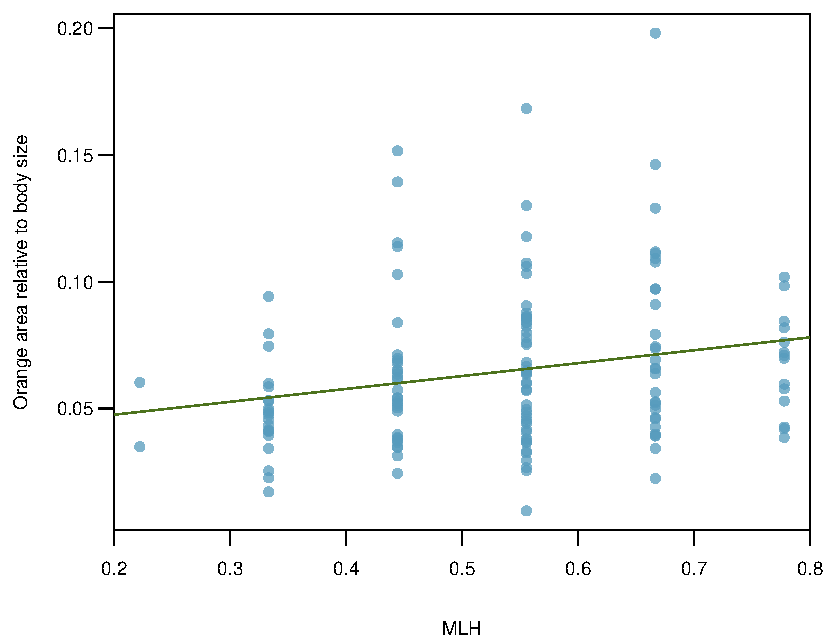
\includegraphics[width=0.32\textwidth]{ch_simple_linear_regression_oi_biostat/figures/eoce/guppies/guppies_orange_mlh.pdf}
	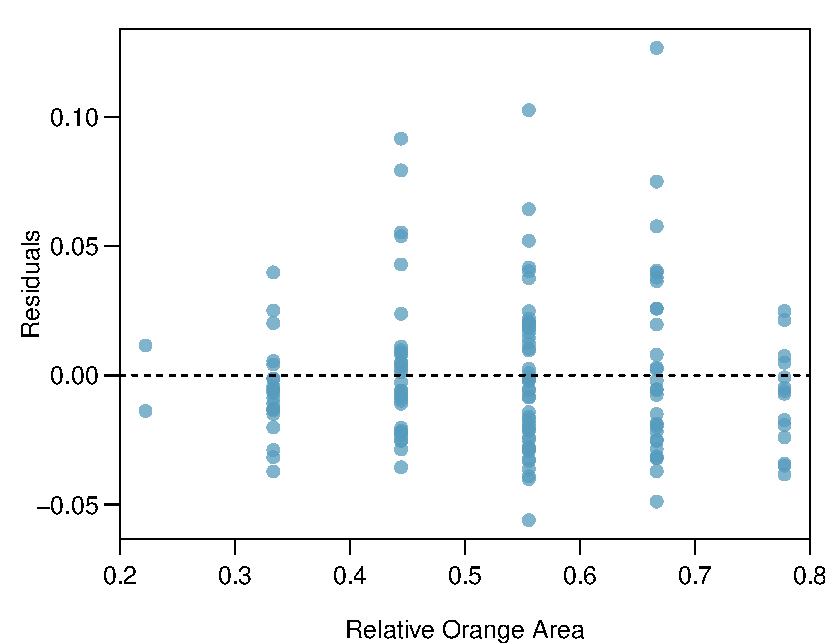
\includegraphics[width=0.32\textwidth]{ch_simple_linear_regression_oi_biostat/figures/eoce/guppies/guppies_mlh_resid.pdf}	
	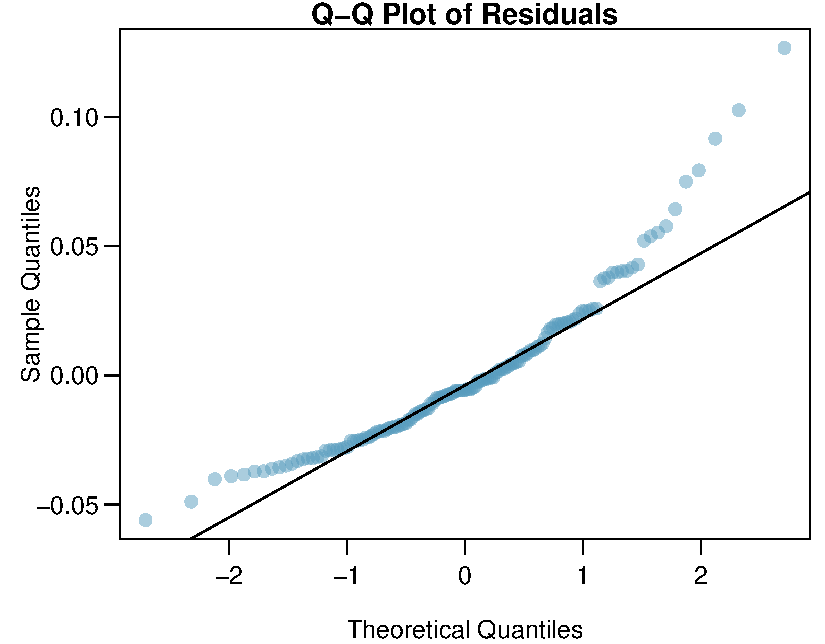
\includegraphics[width=0.32\textwidth]{ch_simple_linear_regression_oi_biostat/figures/eoce/guppies/guppies_mlh_qq.pdf}
\end{center}	
	
\begin{parts}
	\item Based on the plot of MLH versus relative orange area, describe the nature of the association in language accessible to a general audience.
	\item Comment on whether the assumptions of linearity and constant variability are reasonably met.
	\item Comment on whether the residuals are approximately normally distributed.
\end{parts}	
		
}{}

\textD{\newpage}

% 21 oi_biostat

\eoce{\qt{Diamond prices, Part II\label{diamonds_binary}} Exercise~\ref{diamonds_two_group} introduced data on the price of diamonds based on whether a diamond is 0.99 carats or 1 carat. Based on the summary statistics, write an estimated model equation predicting price from a binary indicator of carat weight. Be sure to clearly define the variables used in the model. \\
	
\vspace{1mm}	

		\begin{tabular}{l c c }
			\hline
			& 0.99 carats	 	& 1 carat\\
			\hline	
			Mean 	& \$ 44.51			& \$ 56.81			 \\
			SD		& \$ 13.32			&\$ 16.13			 \\
			n		&23				    & 23 \\
			\hline
		\end{tabular}
}{}

% 22 oi_biostat

\eoce{\qt{Avian influenza, Part II\label{avian_influenza_binary}} Exercise~\ref{avian_influenza_two_group} introduced data from an analysis investigating whether hatch weights between transgenic and non-transgenic chicks differ. \\
	
\vspace{1mm}	
	
	\begin{tabular}{l c c}
		\hline
		& transgenic chicks	(g) & non-transgenic chicks (g) \\
		\hline	
		$\bar{x}$ &45.14			& 44.99 		    \\
		$s$		  &3.32			&  4.57		    \\
		$n$		  &54				& 54			\\
		\hline
	\end{tabular}	
	
 \begin{parts}
 	\item Write an estimated least squares regression line for a model predicting hatch weight from chick type, where non-transgenic chicks are the reference group; i.e., the group for which the binary predictor takes on value \texttt{0}.
 	\item Write an estimated least squares regression line for a model predicting hatch weight from chick type, where transgenic chicks are the reference group.
 \end{parts}
	
}{}


\textD{\newpage}


\subsection{Statistical inference with regression}

% 23 ODD (OI4, 8.31)

\eoce{\qt{Body measurements, Part IV\label{body_measurements_weight_height_inf}} 
The scatterplot and least squares summary below show the relationship 
between weight measured in kilograms and height measured in centimeters 
of 507 physically active individuals.

\noindent\begin{minipage}[c]{0.4\textwidth}
\begin{center}
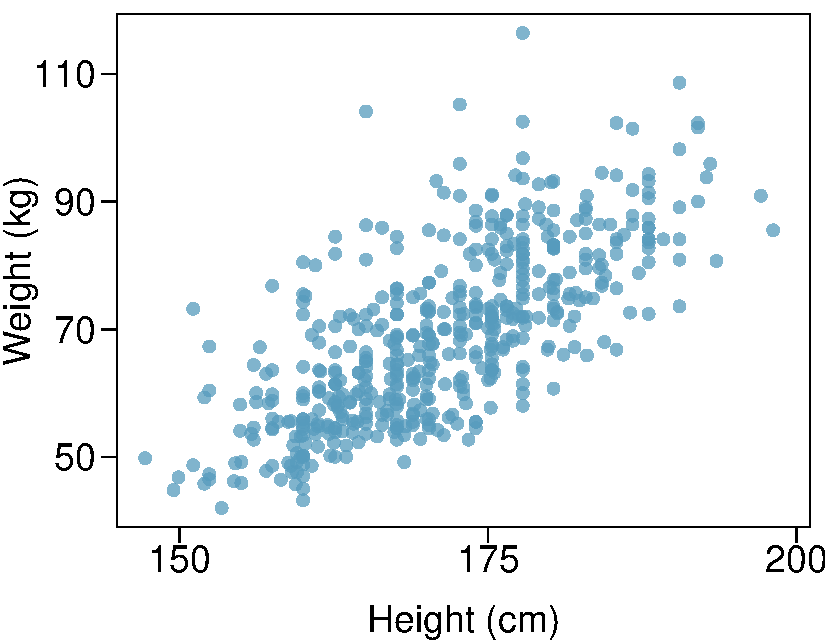
\includegraphics[width=\textwidth]{ch_simple_linear_regression_oi_biostat/figures/eoce/body_measurements_weight_height_inf/body_measurements_weight_height.pdf}
\end{center}
\end{minipage}
\begin{minipage}[c]{0.6\textwidth}
{\scriptsize
\begin{center}
\begin{tabular}{rrrrr}
    \hline
            & Estimate  & Std. Error    & t value   & Pr($>$$|$t$|$) \\ 
    \hline
(Intercept) & -105.0113 & 7.5394        & -13.93    & 0.0000 \\ 
height      & 1.0176    & 0.0440        & 23.13     & 0.0000 \\
    \hline
\end{tabular}
\end{center}
}
\end{minipage}
\begin{parts}
\item Describe the relationship between height and weight.
\item Write the equation of the regression line. Interpret the slope 
and intercept in context.
\item Do the data provide strong evidence that an increase in height 
is associated with an increase in weight? State the null and alternative 
hypotheses, report the p-value, and state your conclusion.
\item The correlation coefficient for height and weight is 0.72. 
Calculate $R^2$ and interpret it in context.
\end{parts}
}{}

\textC{\pagebreak}


% 24 EVEN (OI4, 8.32)

\eoce{\qt{Beer and blood alcohol content\label{beer_blood_alcohol_inf}} 
Many people believe that gender, 
weight, drinking habits, and many other factors are much more important 
in predicting blood alcohol content (BAC) than simply considering the 
number of drinks a person consumed. Here we examine data from sixteen 
student volunteers at Ohio State University who each drank a randomly 
assigned number of cans of beer. These students were evenly divided 
between men and women, and they differed in weight and drinking habits. 
Thirty minutes later, a police officer measured their blood alcohol 
content (BAC) in grams of alcohol per deciliter of blood.
\footfullcite{Malkevitc+Lesser:2008} The scatterplot and regression 
table summarize the findings.

\noindent\begin{minipage}[c]{0.4\textwidth}
\begin{center}
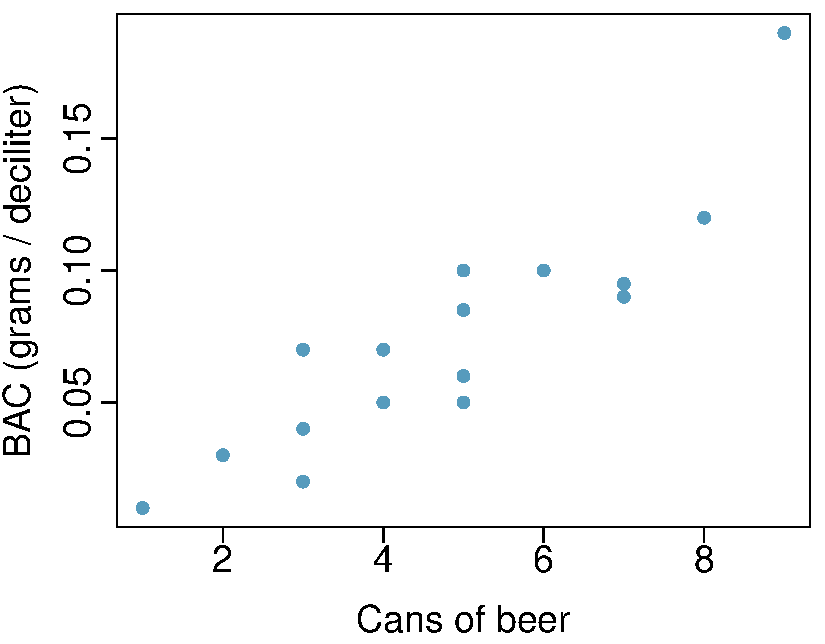
\includegraphics[width=\textwidth]{ch_simple_linear_regression_oi_biostat/figures/eoce/beer_blood_alcohol_inf/beer_blood_alcohol.pdf}
\end{center}
\end{minipage}
\begin{minipage}[c]{0.6\textwidth}
{\scriptsize
\begin{center}
\begin{tabular}{rrrrr}
    \hline
            & Estimate  & Std. Error    & t value   & Pr($>$$|$t$|$) \\ 
    \hline
(Intercept) & -0.0127   & 0.0126        & -1.00     & 0.3320 \\ 
beers       & 0.0180    & 0.0024        & 7.48      & 0.0000 \\ 
    \hline
\end{tabular}
\end{center}
}
\end{minipage}
\begin{parts}
\item Describe the relationship between the number of cans of beer 
and BAC.
\item Write the equation of the regression line. Interpret the slope 
and intercept in context.
\item Do the data provide strong evidence that drinking more cans of 
beer is associated with an increase in blood alcohol? State the null 
and alternative hypotheses, report the p-value, and state your 
conclusion.
\item The correlation coefficient for number of cans of beer and BAC 
is 0.89. Calculate $R^2$ and interpret it in context.
\item Suppose we visit a bar, ask people how many drinks they have had, 
and also take their BAC. Do you think the relationship between number 
of drinks and BAC would be as strong as the relationship found in the 
Ohio State study?
\end{parts}
}{}

\textD{\newpage}

% 25 ODD (OI4, 8.33) edited, shown as Part II in OI4

\eoce{\qt{Husbands and wives, Part I\label{husbands_wives_height_inf}} The 
scatterplot below summarizes husbands' and wives' heights in a random 
sample of 170 married couples in Britain, where both partners' ages are 
below 65 years. Summary output of the least squares fit for predicting 
wife's height from husband's height is also provided in the table.

\noindent\begin{minipage}[c]{0.4\textwidth}
\begin{center}
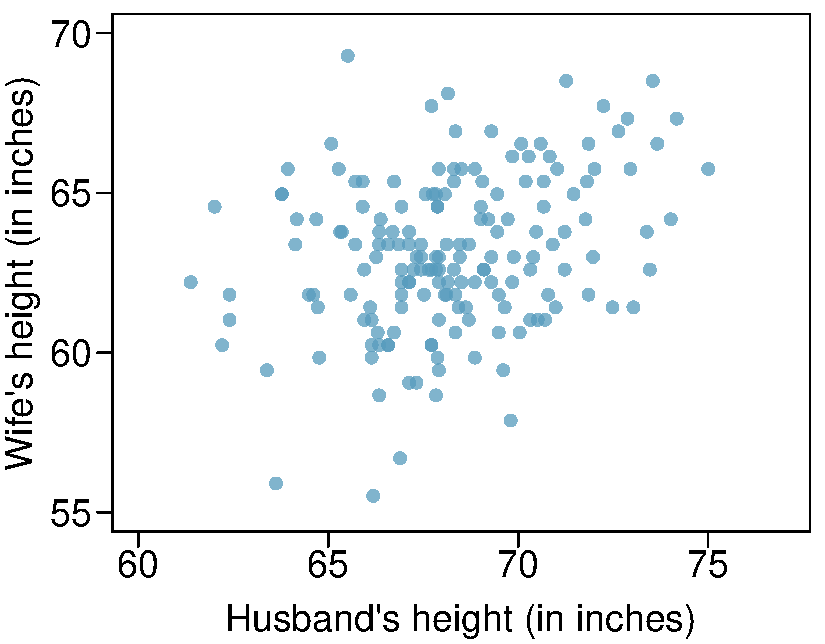
\includegraphics[width=\textwidth]{ch_simple_linear_regression_oi_biostat/figures/eoce/husbands_wives_height_inf_2s/husbands_wives_height_inf_2s}
\end{center}
\end{minipage}
\begin{minipage}[c]{0.6\textwidth}
{\scriptsize
\begin{center}
\begin{tabular}{rrrrr}
    \hline
                    & Estimate  & Std. Error    & t value   & Pr($>$$|$t$|$) \\ 
    \hline
(Intercept)         & 43.5755   & 4.6842        & 9.30      & 0.0000 \\ 
height\_\hspace{0.3mm}husband   & 0.2863    & 0.0686        & 4.17      & 0.0000 \\ 
    \hline
\end{tabular}
\end{center}
}
\end{minipage}
\begin{parts}
\item Is there strong evidence that taller men marry taller women? 
State the hypotheses and include any information used to conduct the test.
\item Write the equation of the regression line for predicting wife's 
height from husband's height.
\item Interpret the slope and intercept in the context of the application.
\item Given that $R^2 = 0.09$, what is the correlation of heights 
in this data set?
\item You meet a married man from Britain who is 5'9" (69 inches). 
What would you predict his wife's height to be? How reliable is this 
prediction?
\item You meet another married man from Britain who is 6'7" (79 inches). 
Would it be wise to use the same linear model to predict his wife's 
height? Why or why not?
\item Is there statistically significant evidence of an association between husband height and wife height based on these data? Explain your answer.
\item Would you expect a 95\% confidence interval for husband height to contain 0? Explain your answer.
\end{parts}
}{}

% 26 EVEN (OI4, 8.42)

\eoce{\qt{Helmets and lunches\label{helmet_lunch}}
	The scatterplot shows the 
	relationship between socioeconomic status measured as the percentage of 
	children in a neighborhood receiving reduced-fee lunches at school 
	({\tt lunch}) and the percentage of bike riders in the neighborhood 
	wearing helmets ({\tt helmet}). The average percentage of children 
	receiving reduced-fee lunches is 30.8\% with a standard deviation 
	of 26.7\% and the average percentage of bike riders wearing helmets 
	is 38.8\% with a standard deviation of 16.9\%.
	
	\noindent\begin{minipage}[c]{0.5\textwidth}
		{\raggedright\begin{parts}
				\item If the $R^2$ for the least-squares regression line for these 
				data is $72\%$, what is the correlation between {\tt lunch} 
				and {\tt helmet}?
				\item Calculate the slope and intercept for the least-squares regression 
				line for these data.
				\item Interpret the intercept of the least-squares regression line in 
				the context of the application.
				\item Interpret the slope of the least-squares regression line in the 
				context of the application.
				\item What would the value of the residual be for a neighborhood where 
				40\% of the children receive reduced-fee lunches and 40\% of the bike 
				riders wear helmets? Interpret the meaning of this residual in the context 
				of the application.
		\end{parts}}
	\end{minipage}
	\begin{minipage}[c]{0.05\textwidth}
		$\:$ \\
	\end{minipage}
	\begin{minipage}[c]{0.42\textwidth}
		\begin{center}
			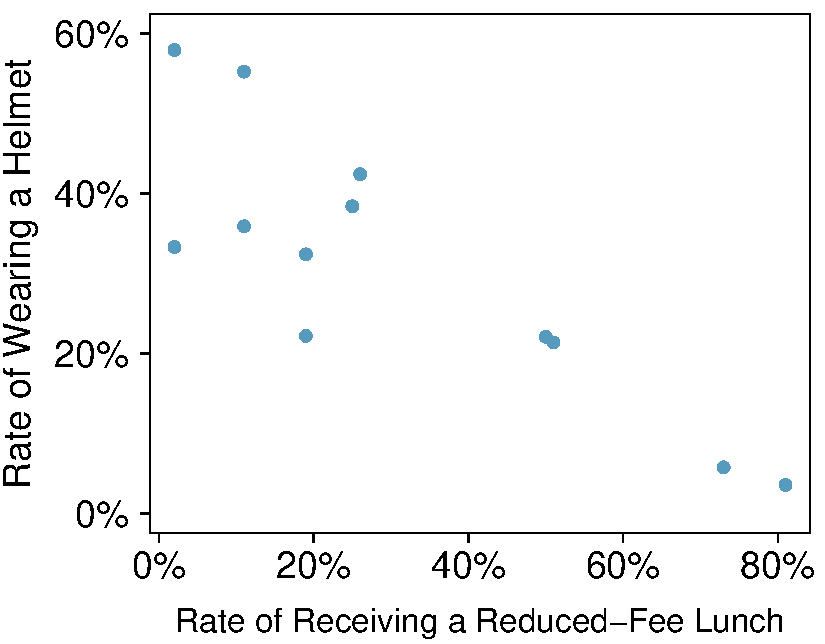
\includegraphics[width=\textwidth]{ch_simple_linear_regression_oi_biostat/figures/eoce/helmet_lunch/helmet_lunch.pdf} \\
		\end{center}
	\end{minipage}
}{}

\textD{\newpage}

% 27 ODD (OI4, 8.39) shows as Part III in OI4

\eoce{\qt{Husbands and wives, Part II\label{husbands_wives_age_inf}}
Exercise~\ref{husbands_wives_height_inf} presents a scatterplot displaying the 
relationship between husbands' and wives' ages in a random sample of 
170 married couples in Britain, where both partners' ages are below 65 
years. Given below is summary output of the least squares fit for 
predicting wife's age from husband's age.

\noindent\begin{minipage}[c]{0.4\textwidth}
\begin{center}
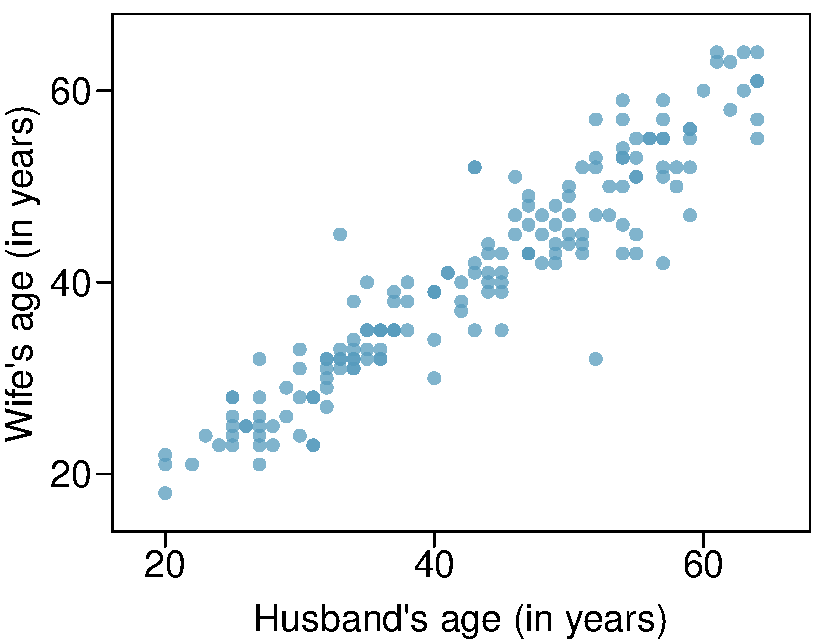
\includegraphics[width=\textwidth]{ch_simple_linear_regression_oi_biostat/figures/eoce/husbands_wives_age_inf/husbands_wives_age.pdf}
\end{center}
\end{minipage}
\begin{minipage}[c]{0.6\textwidth}
{\scriptsize
\begin{center}
\begin{tabular}{rrrrr}
  \hline
                & Estimate  & Std. Error    & t value   & Pr($>$$|$t$|$) \\ 
  \hline
(Intercept)     & 1.5740    & 1.1501        & 1.37      & 0.1730 \\ 
age\_\hspace{0.3mm}husband  & 0.9112    & 0.0259        & 35.25     & 0.0000 \\ 
   \hline
\multicolumn{5}{r}{$df = 168$} \\
\end{tabular}
\end{center}
}
\end{minipage}
\begin{parts}
\item We might wonder, is the age difference between husbands and 
wives consistent across ages? If this were the case, then the slope 
parameter would be $\beta_1 = 1$. Use the information above to evaluate 
if there is strong evidence that the difference in husband and wife ages 
differs for different ages.
\item Write the equation of the regression line for predicting wife's 
age from husband's age.
\item Interpret the slope and intercept in context.
\item Given that $R^2 = 0.88$, what is the correlation of ages in 
this data set?
\item You meet a married man from Britain who is 55 years old. What 
would you predict his wife's age to be? How reliable is this prediction?
\item You meet another married man from Britain who is 85 years old. 
Would it be wise to use the same linear model to predict his wife's 
age? Explain.
\end{parts}
}{}

% 28 oi_biostat

\eoce{\qt{Guppies, Part V\label{guppies_inference}} Exercise~\ref{guppies_mlh} introduced a linear model for predicting relative orange area from proportion of loci that are heterozygous (MLH). Relative orange area refers to the percentage of the body that is orange (rather than a different color).

\begin{center}
	\begin{tabular}{rrrrr}
		\hline
		& Estimate  & Std. Error    & t value   & Pr($>$$|$t$|$) \\ 
		\hline
		(Intercept)     & 0.037   & 0.010       & 3.68     & 0.0033 \\ 
		MLH  & 0.051    & 0.018       & 2.77    & 0.0063 \\ 
		\hline
		\multicolumn{5}{r}{$df = 145$} \\
	\end{tabular}
\end{center}

\begin{parts}
	
	\item Write the estimated model equation.
	
	\item What is the predicted mean relative orange area for a guppy that is heterozygous at 8 out of 9 loci?
	
	\item Based on the linear model, how much does mean relative orange area differ between a guppy that is heterozygous at 2 loci versus 4 loci (out of 9 total)?
	
	\item Conduct a hypothesis test to determine whether relative orange area is significantly associated with MLH. Do the results suggest that more elaborate sexual ornaments are associated with increased heterozygosity? Explain.
	
	\item Compute and interpret a 95\% confidence interval for the slope parameter $\beta_1$.
	
\end{parts}

}{}

\textD{\newpage}

% 29 oi_biostat

\eoce{\qt{Age and RFFT score, Part II\label{age_rfft_inf}} The following regression output is for predicting RFFT score of 500 randomly sampled individuals from the PREVEND data based on age (years).
	
\begin{center}
	\begin{tabular}{rrrrr}
		\hline
		& Estimate  & Std. Error    & t value   & Pr($>$$|$t$|$) \\ 
		\hline
		(Intercept)     & 137.55   & 5.02       & 27.42     & 0.000\\ 
		Age  & -1.26    & 0.09      & -14.09    & 0.000 \\ 
		\hline
		\multicolumn{5}{r}{$df = 498$} \\
	\end{tabular}
\end{center}

\begin{parts}
	\item Do these data provide statistically significant evidence at the $\alpha = 0.01$ significance level that age is associated with RFFT score? State the null and alternative hypotheses, report the relevant $p$-value, and state your conclusion.
	\item Compute and interpret a 99\% confidence interval for the population slope.
\end{parts}

}{}

% 30 oi_biostat

\eoce{\qt{Avian influenza, Part III\label{avian_influenza_inf}} Exercise~\ref{avian_influenza_two_group} introduced data from an analysis investigating whether hatch weights between transgenic and non-transgenic chicks differ. Based on the results from conducting the two-group test, explain whether the 95\% confidence interval for the $\beta_1$ parameter in a model predicting hatch weight from a group indicator would contain 0.
}{}

% 31 oi_biostat

\eoce{\qt{Husbands and wives, Part III\label{husbands_wives_age_interval}} Exercise~\ref{husbands_wives_age_inf} introduces data from a random sample of 170 married couples in Britain, where both partners' ages are below 65 years, and fits a model predicting wife's age from husband's age. Wife's age has a mean of 40.68 years, with standard deviation 11.41 years. Husband's age has a mean of 42.92 years, with standard deviation 11.76 years. From software, the residual standard error is $s = 3.95$.

\begin{parts}
	
	\item Use the summary statistics to calculate a 95\% confidence interval for the average age of wives whose husbands are 55 years old.
	
	\item You meet a married man from Britain who is 55 years old.  Predict his wife's age and give a 95\% prediction interval for her age.
	
	\item Repeat parts~(a) and (b) using the approximate formulas for the appropriate standard errors.
	
\end{parts}
}{}


% 32 oi_biostat

\eoce{\qt{Guppies, Part VI\label{guppies_intervals}} The relationship between length and height for 147 male guppies was introduced in Exercise~\ref{guppies_one}, which used the summary statistics to calculate the equation of the least squares line for length as a function of height and estimate the mean length of an adult male guppy with height 180 cm. The estimated residual standard error from this model is $s = 50.93$.
	
	\begin{parts}
		
		\item  Use the summary statistics given in Exercise~\ref{guppies_one} to construct a 95\% confidence interval for the estimated mean length when height is 180 cm.
		
		\item Use a prediction interval based on the summary statistics to estimate the lengths for a new 180 cm guppy that would be more than two standard deviations above and below the estimated mean.
		
		\item Use the approximate formulas for the standard error for a mean and for a prediction to recalculate the intervals in parts~(a) and (b).
		
	\end{parts}
	
}{}